\chapter{对称性与守恒定律}

\lectureoverview{稳定作用量与欧拉--拉格朗日方程是经典力学核心的一半；哈密顿表述则是另一半。这里我们将前半部分展开到足以揭示一个深刻的模式：拉格朗日量的每一个连续对称性都产生一个守恒量。我们将在平移和旋转中发现这一模式，对一般无穷小变换加以证明，然后仔细考察该论证在何处适用、在何处不适用。}

\section{解释物理所需的最低限度数学}

黑板上已有的符号可能看起来有点像薛定谔方程，但那不是今晚的主题。主题是对称性与守恒。若不借助方程，就无法诚实地解释它们之间的联系。这些方程是初等的；关键在于把它们安排得使结构变得可见。《科学美国人》或许会给出结果的名称，但在这里我们要的是物理学家推导它所需的最低限度数学。

引入一个小参数\(\epsilon\)。我们保留正比于\(\epsilon\)的项，舍弃\(O(\epsilon^2)\)。这是一种极限论证的简写，并不是说一个非零实数真的具有零平方。对于普通函数\(f(x,y)\)，
\begin{equation}
  \delta f
  =\frac{\partial f}{\partial x}\,\delta x
   +\frac{\partial f}{\partial y}\,\delta y
   +O(\epsilon^2),
  \label{eq:first-variation-f}
\end{equation}
其中\(\delta x\)和\(\delta y\)都正比于\(\epsilon\)。符号\(\delta f\)表示\(f\)的变化，而不是某个称为\(\delta\)的数与\(f\)的乘积。稳定点满足
\begin{equation}
  \delta f=0
  \qquad\hbox{to first order.}
  \label{eq:stationary-f}
\end{equation}

对于力学路径\(q_i(t)\)，类似的量是作用量
\begin{equation}
  S[q]=\int_{t_1}^{t_2}L(q,\dot q,t)\,dt.
  \label{eq:action-l4}
\end{equation}
在固定端点的情况下对路径作变分，得到
\begin{equation}
  \delta S
  =\int_{t_1}^{t_2}dt\,
   \sum_i\left(
     \frac{\partial L}{\partial q_i}\,\delta q_i
     +\frac{\partial L}{\partial\dot q_i}\,\delta\dot q_i
   \right).
  \label{eq:action-variation-l4}
\end{equation}
出现这两项，是因为改变路径会同时改变其位置和速度。分部积分，连同
\(\delta q_i(t_1)=\delta q_i(t_2)=0\)，把\(\delta S=0\)化为
\begin{equation}
  \frac{d}{dt}\left(\frac{\partial L}{\partial\dot q_i}\right)
  -\frac{\partial L}{\partial q_i}=0.
  \label{eq:el-l4}
\end{equation}

\begin{figure}[htbp]
  \centering
  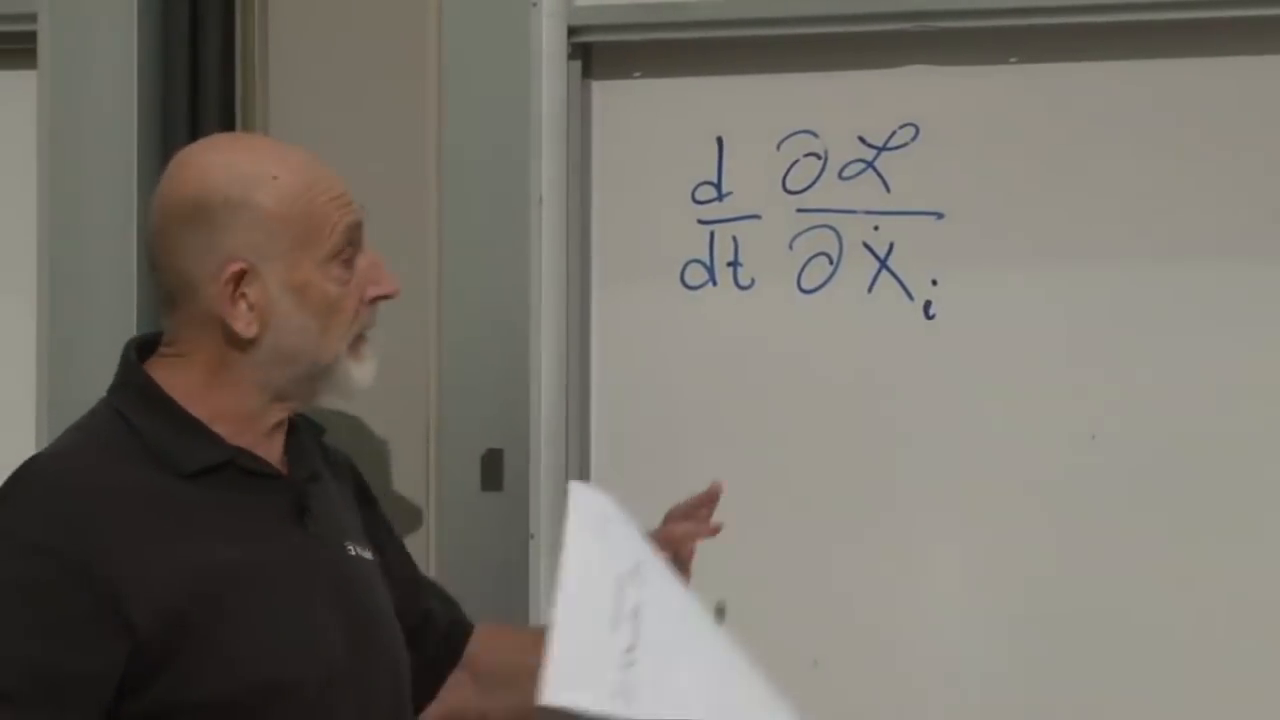
\includegraphics[width=0.76\textwidth]{lecture_04_figure_05.png}
  \caption{作为对称性与守恒出发点的欧拉--拉格朗日方程回顾。}
  \lectureframe{00:09:00}
\end{figure}

正确的说法是\emph{稳定作用量}，而不一定是最小作用量。这一区别将在接近结尾处再次出现。

\section{广义坐标与共轭动量}

笛卡尔位置对于一般力学来说是一种过于狭窄的语言。坐标可以是粒子位置、角度、集体变量或场振幅，因此我们称它们为\(q_i\)。拉格朗日量是对动力学的压缩描述。即便是标准模型，若不用高度浓缩的记号写出，也大约占一页；为每个场分量分别写出运动方程，篇幅会大得多。一个函数\(L\)就把它们全部打包在一起。

与\(q_i\)共轭的动量是
\begin{equation}
  p_i=\frac{\partial L}{\partial\dot q_i}.
  \label{eq:canonical-momentum-l4}
\end{equation}
这就是为什么广义坐标传统上被称为\(q\)：相应的动量是\(p\)，从而给我们\(p\)和\(q\)。在这一记号下，式~\eqref{eq:el-l4}变为
\begin{equation}
  \dot p_i=\frac{\partial L}{\partial q_i}.
  \label{eq:momentum-el-l4}
\end{equation}

对于熟悉的一维粒子，
\begin{equation}
  L=\frac{m\dot x^2}{2}-V(x),
  \qquad
  \frac{\partial L}{\partial\dot x}=m\dot x,
  \label{eq:particle-momentum-l4}
\end{equation}
所以共轭动量就是普通动量。

\begin{figure}[htbp]
  \centering
  \includegraphics[width=0.72\textwidth]{lecture_04_figure_02.png}
  \caption{用来把共轭动量等同于\(m\dot x\)的动能减势能拉格朗日量。}
  \lectureframe{00:14:48}
\end{figure}

如果\(q_i\)不出现在\(L\)中，那么\(\dot p_i=0\)。这是通向守恒律的熟悉的循环坐标途径。真正的联系更为一般，而在证明之前先在例子中发现它是有益的。

\section{在得到解释之前发现的守恒定律}

\subsection{两个坐标与一个分离势}

令两个质量都等于一，并取
\begin{equation}
  L=\frac{\dot q_1^{\,2}+\dot q_2^{\,2}}{2}-V(q_1-q_2).
  \label{eq:separation-lagrangian}
\end{equation}
可以想象直线上有两个粒子。它们的相互作用只依赖于它们的间距。

\begin{figure}[htbp]
  \centering
  \includegraphics[width=0.78\textwidth]{lecture_04_figure_03.png}
  \caption{双坐标拉格朗日量及其第一个动量方程的开头。}
  \lectureframe{00:18:56}
\end{figure}

用\(V'\)表示对\(V\)的自变量求导，
\begin{align}
  \dot p_1&=-V'(q_1-q_2),
  \notag\\
  \dot p_2&=+V'(q_1-q_2).
  \label{eq:separation-momentum-equations}
\end{align}
第二个符号反转，是因为增大\(q_2\)会减小\(q_1-q_2\)。

\begin{classroomqa}
  \audiencequestion{第一个动量方程中是否应包含\(V'\)，它的负号从何而来？
  \lecturetimestamp{00:20:52--00:21:35}}
  \lecturerresponse{欧拉--拉格朗日方程说的是
  \(\dot p_1=\partial L/\partial q_1\)，而不是拉格朗日量为零。由于\(L=T-V\)，对\(q_1\)求导给出
  \(-V'\)。对\(q_2\)求导又从\(q_1-q_2\)提供一个负号，所以第二个方程中有\(+V'\)。}
\end{classroomqa}

\begin{figure}[htbp]
  \centering
  \includegraphics[width=0.78\textwidth]{lecture_04_figure_04.png}
  \caption{\(p_1\) 方程中带符号敏感的导数；\(p_2\) 方程则取相反的符号。}
  \lectureframe{00:20:41}
\end{figure}

将式~\eqref{eq:separation-momentum-equations}相加，得到
\begin{equation}
  \frac{d}{dt}(p_1+p_2)=0.
  \label{eq:total-p-conserved}
\end{equation}
我们已找到一个守恒量，但尚未解释它为何存在。

\subsection{一个不那么明显的线性组合}

现在令
\begin{equation}
  L=\frac{\dot q_1^{\,2}+\dot q_2^{\,2}}{2}
    -V(Aq_1+Bq_2),
  \label{eq:ab-lagrangian}
\end{equation}
其中 \(A\) 与 \(B\) 为常数。于是
\begin{align}
  \dot p_1&=-A\,V'(Aq_1+Bq_2),
  \notag\\
  \dot p_2&=-B\,V'(Aq_1+Bq_2).
  \label{eq:ab-momentum-equations}
\end{align}
将第一个方程乘以 \(B\)，第二个方程乘以 \(A\)，再相减，
即可消去力项：
\begin{equation}
  \frac{d}{dt}(Bp_1-Ap_2)=0.
  \label{eq:ab-conserved}
\end{equation}

\begin{figure}[htbp]
  \centering
  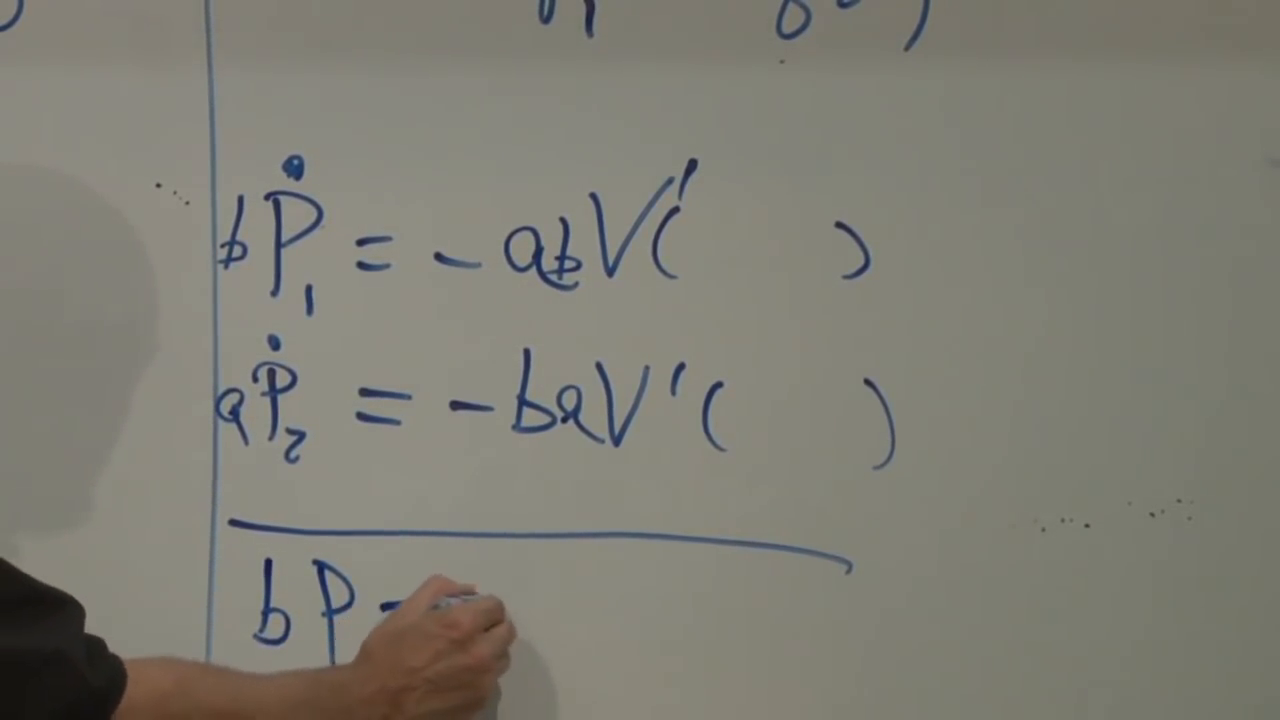
\includegraphics[width=0.78\textwidth]{lecture_04_figure_06.png}
  \caption{加权后的动量方程，其力项在 \(Bp_1-Ap_2\) 中相消。}
  \lectureframe{00:24:20}
\end{figure}

\begin{classroomqa}
  \audiencequestion{像 \(A\) 和 \(B\) 这样的常数，在物理上可能来自何处？\lecturetimestamp{00:25:09--00:30:15}}
  \lecturerresponse{考虑两个质量分别为 \(m\) 和 \(M\) 的粒子：
  \[
    L=\frac{m\dot X^2}{2}+\frac{M\dot Y^2}{2}-V(X-Y).
  \]
  重新标度到 \(Q_1=\sqrt m\,X\) 和 \(Q_2=\sqrt M\,Y\)。动能项
  变为 \((\dot Q_1^2+\dot Q_2^2)/2\)，而势能依赖于
  \(Q_1/\sqrt m-Q_2/\sqrt M\)。因此，不相等的质量自然地成为线性组合中的
  系数。将 \(Q_2\) 替换为 \(-Q_2\)
  会把所显示的减号变为加号，而不改变其动能平方项。}
\end{classroomqa}

\begin{figure}[htbp]
  \centering
  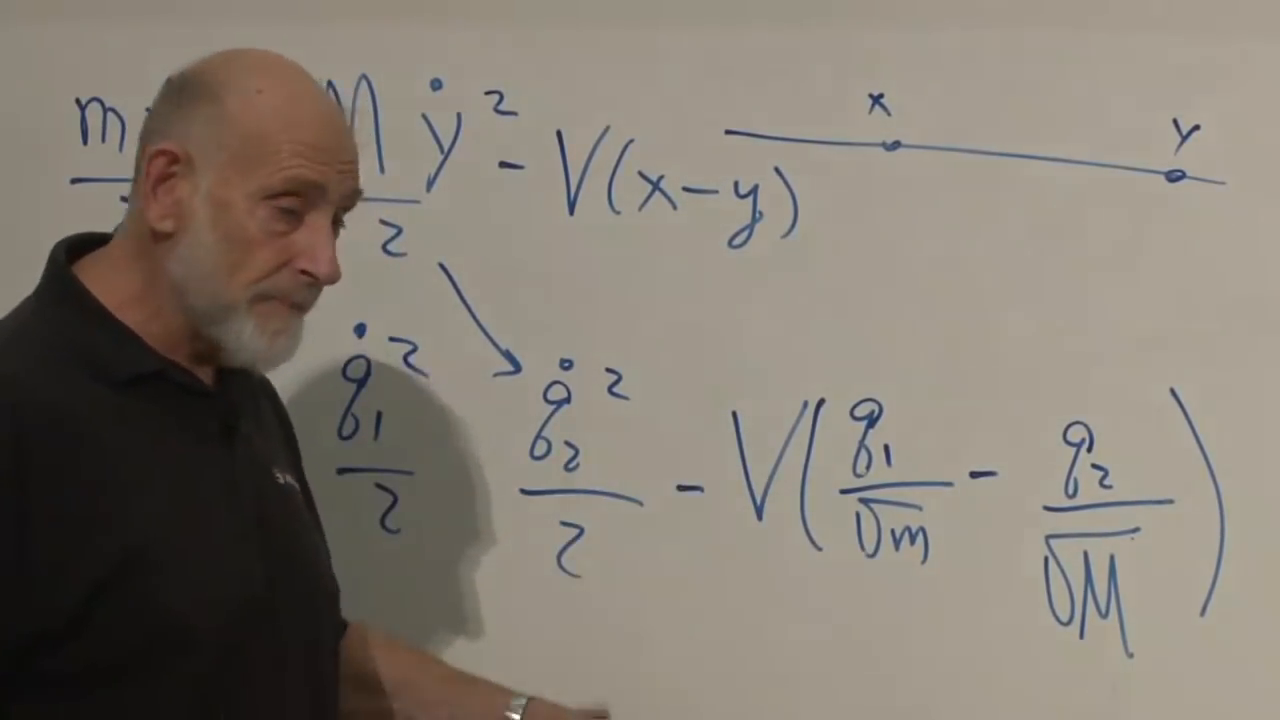
\includegraphics[width=0.82\textwidth]{lecture_04_figure_07.png}
  \caption{质量加权坐标简化了动能，同时把质量因子移入势能。}
  \lectureframe{00:28:40}
\end{figure}

\begin{classroomqa}
  \audiencequestion{这是否表明，守恒量可以在没有循环坐标的情况下存在？\lecturetimestamp{00:31:13--00:31:58}}
  \lecturerresponse{按所写变量来看，并不存在 \emph{明显的} 循环坐标。变量变换或许能揭示出一个，但在这里寻找它并非有用的视角。对称性论证将直接识别出守恒组合。}
\end{classroomqa}

\section{我们所说的对称性是什么意思}

\subsection{平移}

从单位质量的自由粒子开始，
\begin{equation}
  L=\frac{\dot q^2}{2}.
  \label{eq:free-unit-l4}
\end{equation}
将其历史中的每一点平移同一个常数：
\begin{equation}
  q'(t)=q(t)+\epsilon.
  \label{eq:free-translation}
\end{equation}
由于 \(\epsilon\) 与时间无关，\(\dot q'=\dot q\)，因此
\(\delta L=0\)。这种不变性就是平移对称性。

有两种等价的图景。被动地看，移动坐标原点而保持物体固定。主动地看，保持坐标轴固定而移动物体。主动的语言将证明更不易混淆：移动物理构型，并问 \(L\) 是否察觉。

对于式~\eqref{eq:separation-lagrangian}，平移两个坐标：
\begin{equation}
  \delta q_1=\epsilon,
  \qquad
  \delta q_2=\epsilon.
  \label{eq:common-translation}
\end{equation}
速度不变，\(q_1-q_2\) 也不变。

\begin{figure}[htbp]
  \centering
  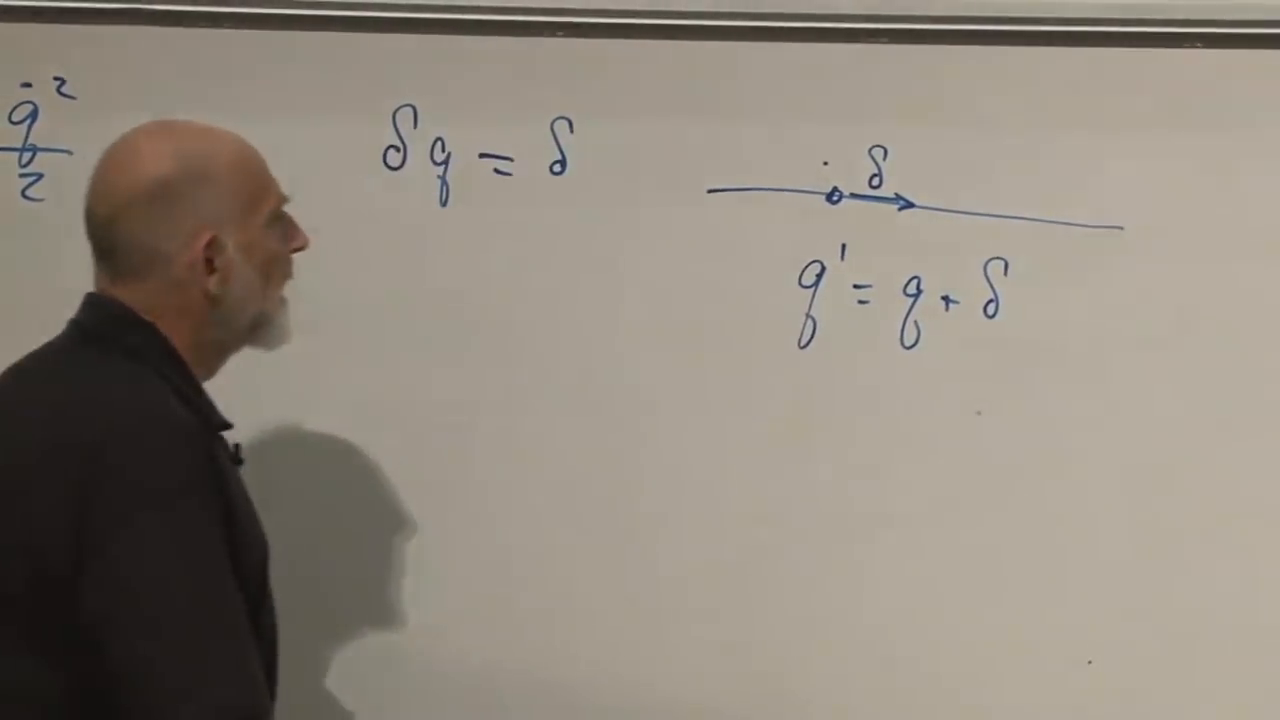
\includegraphics[width=0.78\textwidth]{lecture_04_figure_08.png}
  \caption{共同的平移使两个坐标的间隔保持不变。}
  \lectureframe{00:35:30}
\end{figure}

对于式~\eqref{eq:ab-lagrangian}，使用不那么明显的变换
\begin{equation}
  \delta q_1=B\epsilon,
  \qquad
  \delta q_2=-A\epsilon.
  \label{eq:ab-transformation}
\end{equation}
速度同样不变，而
\begin{equation}
  \delta(Aq_1+Bq_2)=AB\epsilon-BA\epsilon=0.
  \label{eq:ab-invariant-argument}
\end{equation}
因此这个变换是一种对称性。

\begin{figure}[htbp]
  \centering
  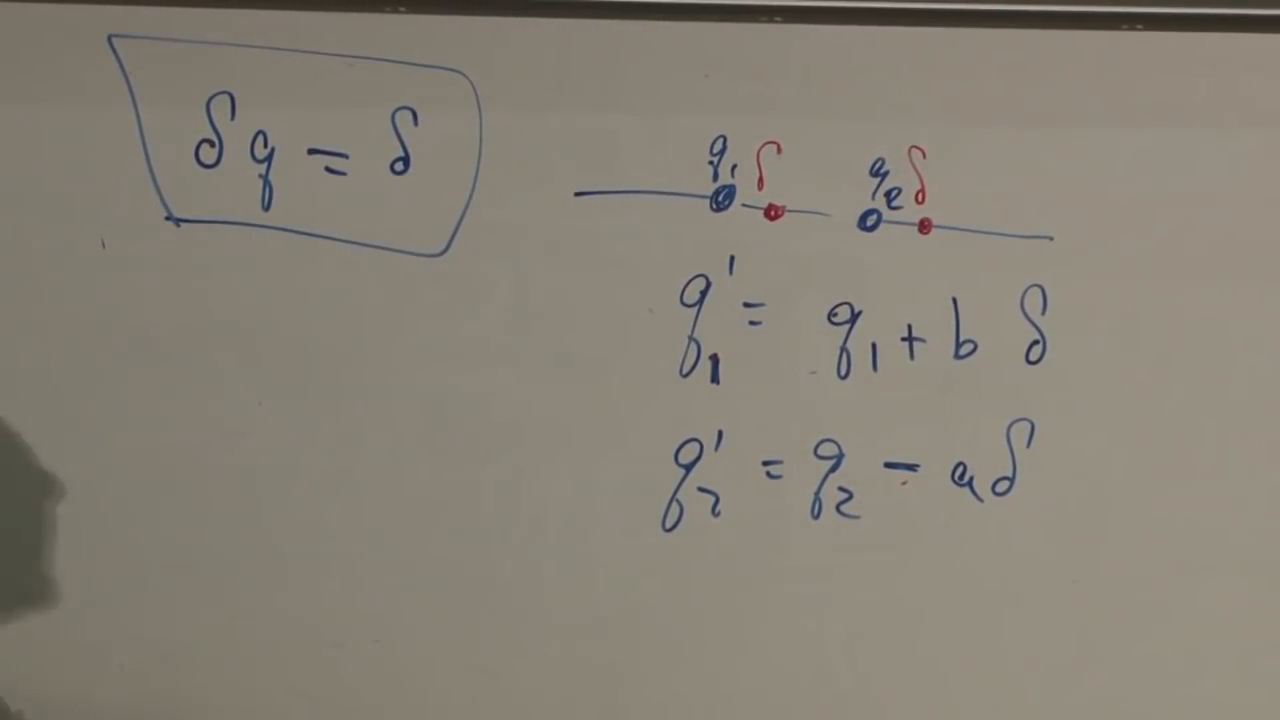
\includegraphics[width=0.80\textwidth]{lecture_04_figure_09.png}
  \caption{保持 \(Aq_1+Bq_2\) 不变的非对称平移。}
  \lectureframe{00:40:20}
\end{figure}

\begin{classroomqa}
  \audiencequestion{这些系数是否编码了质量，从而使守恒量成为通常的质心动量？
  \lecturetimestamp{00:42:25--00:42:45}}
  \lecturerresponse{是的。在质量加权变量中，对称性和守恒组合看起来是非对称的。变换回 \(X\) 和
  \(Y\)，即可恢复通常的同时平移和总动量。}
\end{classroomqa}

\subsection{旋转}

考虑平面中的一个粒子，
\begin{equation}
  L=\frac{m}{2}(\dot x^2+\dot y^2)-V(x^2+y^2).
  \label{eq:central-lagrangian-l4}
\end{equation}
这是一个中心势。我们比较两个彼此相对旋转的固定坐标系；坐标轴并不随时间旋转。取一个
一致的取向，
\begin{align}
  x'&=x\cos\theta+y\sin\theta,
  \notag\\
  y'&=-x\sin\theta+y\cos\theta.
  \label{eq:finite-rotation-l4}
\end{align}

\begin{figure}[htbp]
  \centering
  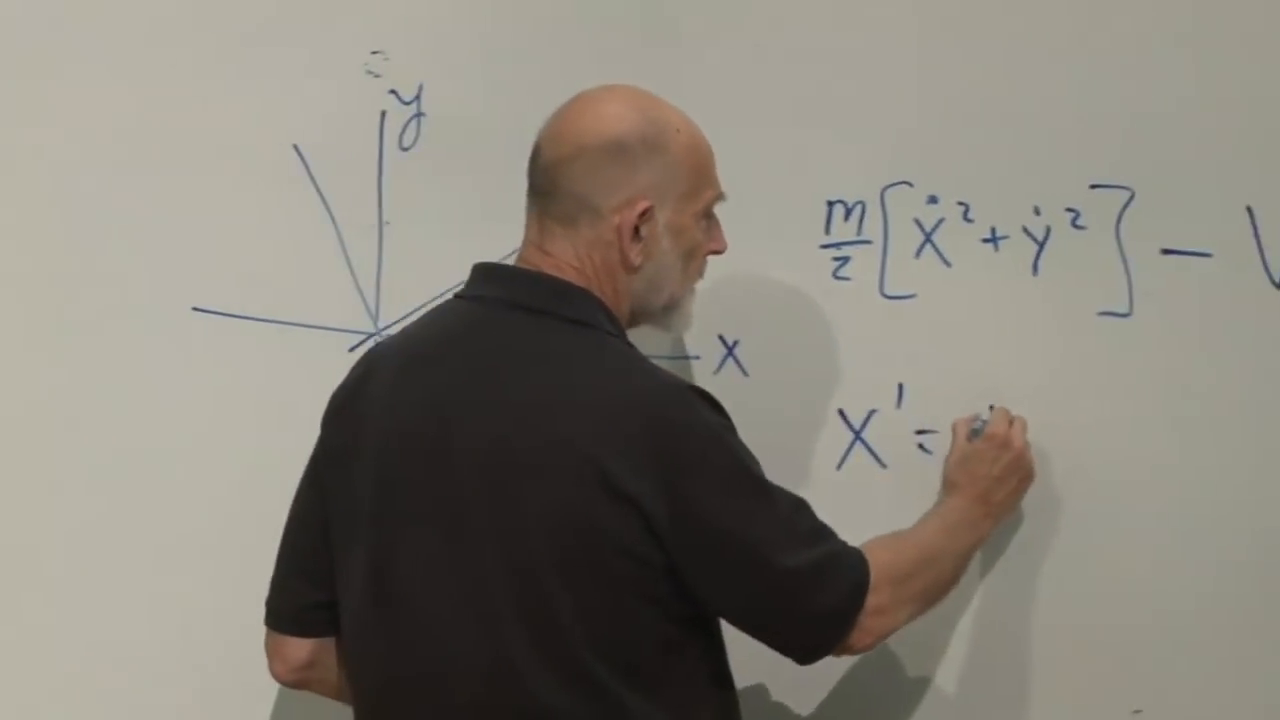
\includegraphics[width=0.82\textwidth]{lecture_04_figure_10.png}
  \caption{中心势拉格朗日量以及由旋转相联系的两个固定笛卡儿坐标系。}
  \lectureframe{00:45:40}
\end{figure}

令 \(\theta=\epsilon\) 并保留一阶项：
\begin{equation}
  \cos\epsilon=1+O(\epsilon^2),
  \qquad
  \sin\epsilon=\epsilon+O(\epsilon^3).
  \label{eq:small-angle-l4}
\end{equation}
无穷小旋转为
\begin{align}
  \delta x&=y\epsilon,
  &\delta y&=-x\epsilon,
  \notag\\
  \delta\dot x&=\dot y\epsilon,
  &\delta\dot y&=-\dot x\epsilon.
  \label{eq:infinitesimal-rotation-l4}
\end{align}

\begin{figure}[htbp]
  \centering
  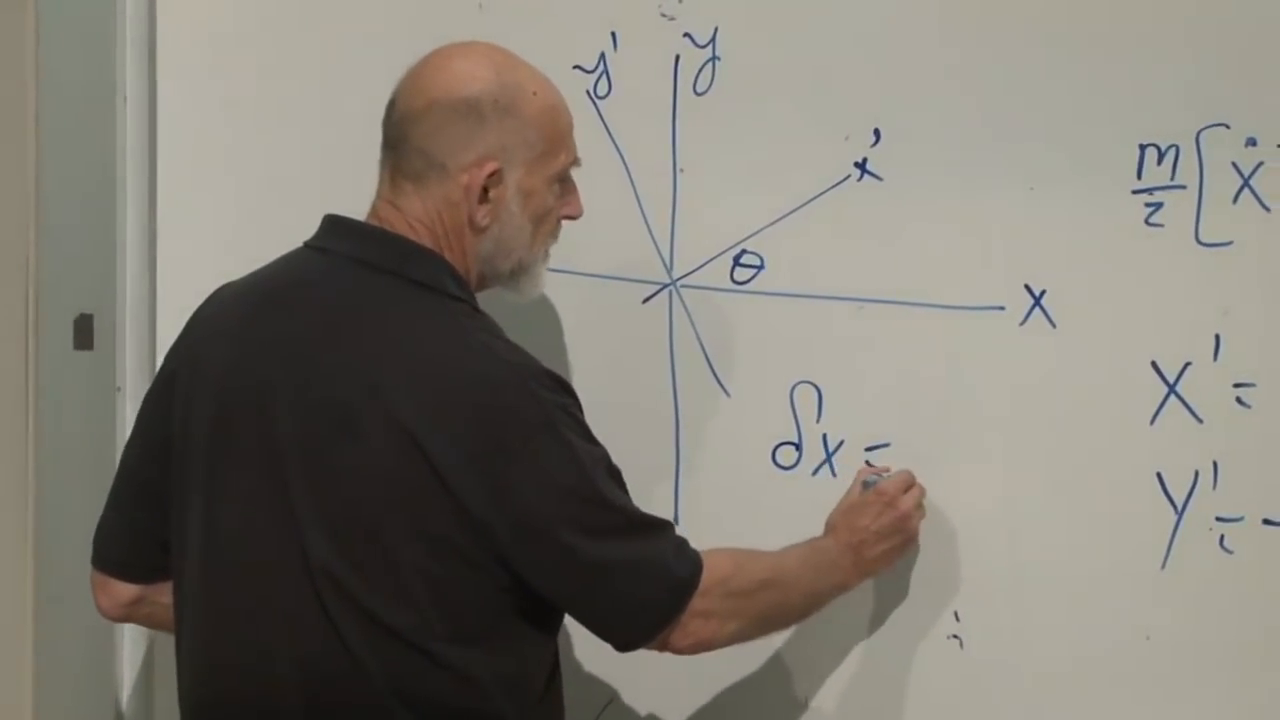
\includegraphics[width=0.82\textwidth]{lecture_04_figure_11.png}
  \caption{坐标与速度的无穷小旋转。}
  \lectureframe{00:49:50}
\end{figure}

与平移不同，\(x\) 改变的量依赖于 \(y\)，而
\(y\) 改变的量依赖于 \(x\)。尽管如此，
\begin{align}
  \delta(x^2+y^2)
  &=2x\,\delta x+2y\,\delta y=0,
  \notag\\
  \delta(\dot x^2+\dot y^2)
  &=2\dot x\,\delta\dot x+2\dot y\,\delta\dot y=0.
  \label{eq:rotation-invariants-l4}
\end{align}
势能项和动能项都不变。

\begin{figure}[htbp]
  \centering
  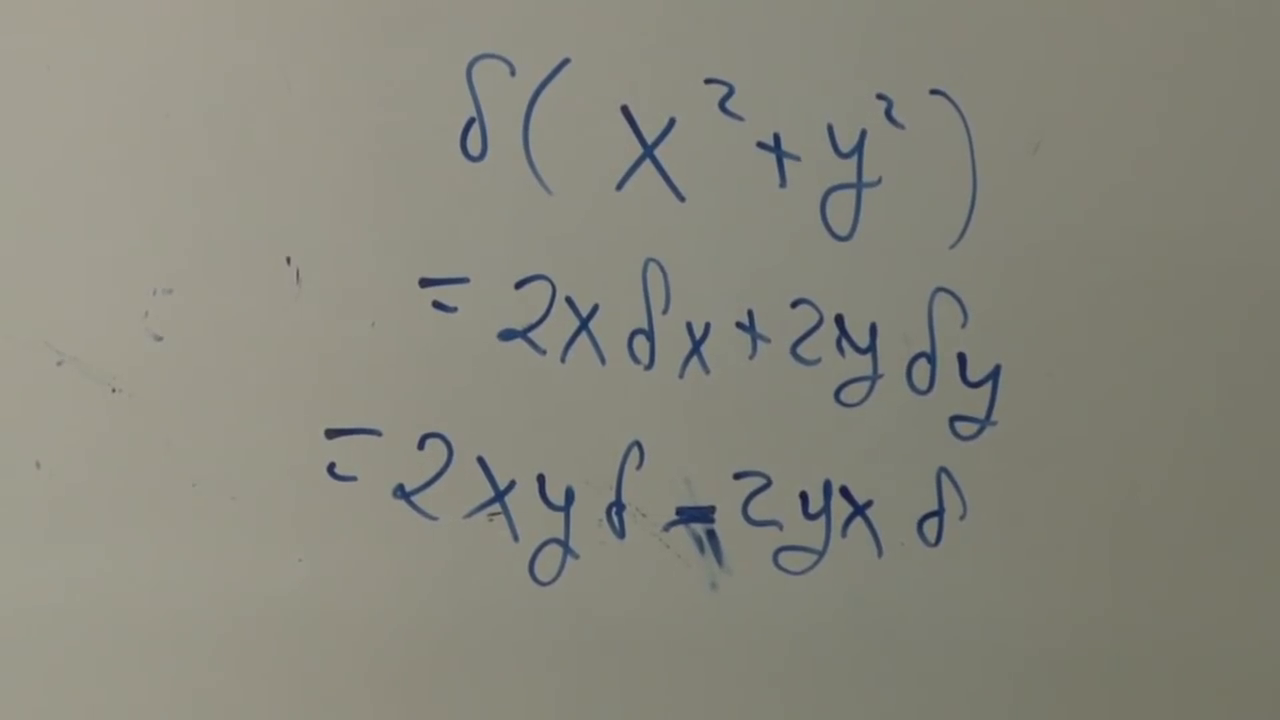
\includegraphics[width=0.76\textwidth]{lecture_04_figure_12.png}
  \caption{证明半径平方在旋转下不变的一阶相消。}
  \lectureframe{00:53:20}
\end{figure}

\section{一般守恒定理}

平移和旋转的例子有一个共同形式。设一个连续无穷小变换为
\begin{equation}
  \delta q_i=\epsilon f_i(q),
  \qquad
  \delta\dot q_i=\frac{d}{dt}\delta q_i,
  \label{eq:general-infinitesimal-symmetry}
\end{equation}
其中 \(\epsilon\) 与时间无关，而 \(f_i\) 可以依赖于所有坐标。

\begin{figure}[htbp]
  \centering
  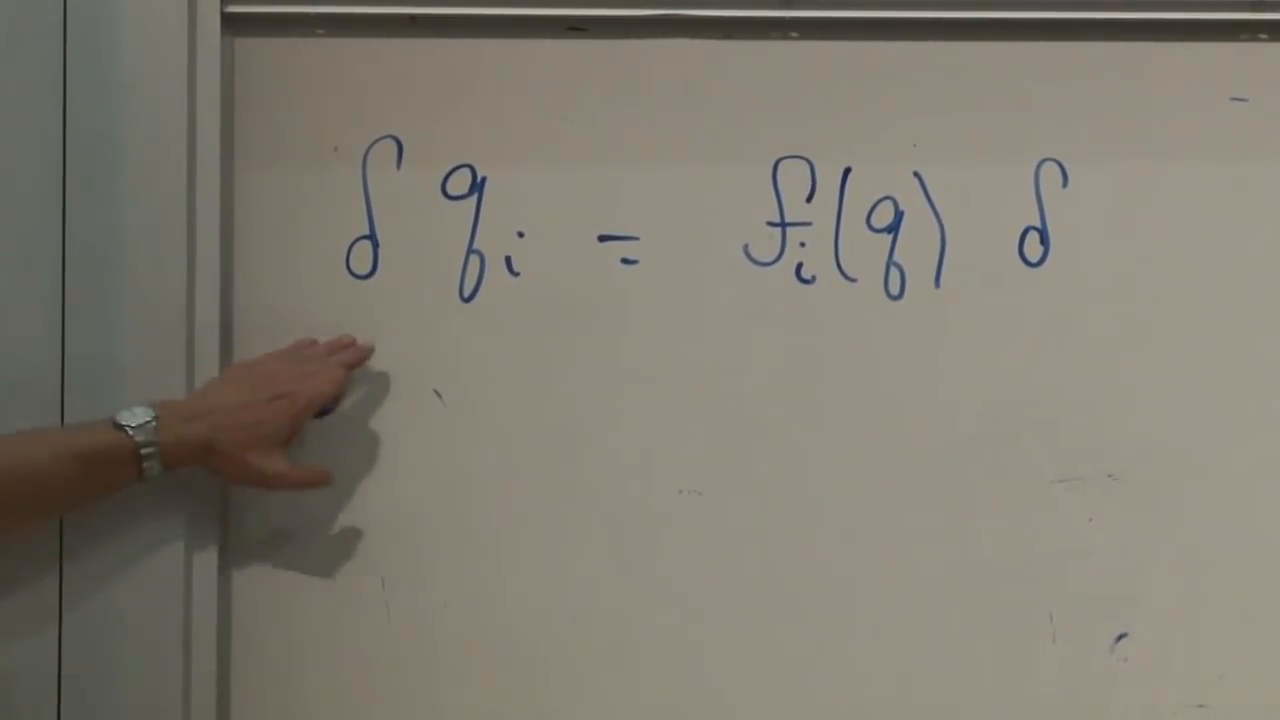
\includegraphics[width=0.78\textwidth]{lecture_04_figure_13.png}
  \caption{一般的无穷小位移场
  \(\delta q_i=\epsilon f_i(q)\)。}
  \lectureframe{00:56:00}
\end{figure}

拉格朗日量的一阶变分为
\begin{equation}
  \delta L
  =\sum_i\left(
    \frac{\partial L}{\partial q_i}\delta q_i
    +\frac{\partial L}{\partial\dot q_i}\delta\dot q_i
  \right).
  \label{eq:delta-l-general}
\end{equation}

\begin{figure}[htbp]
  \centering
  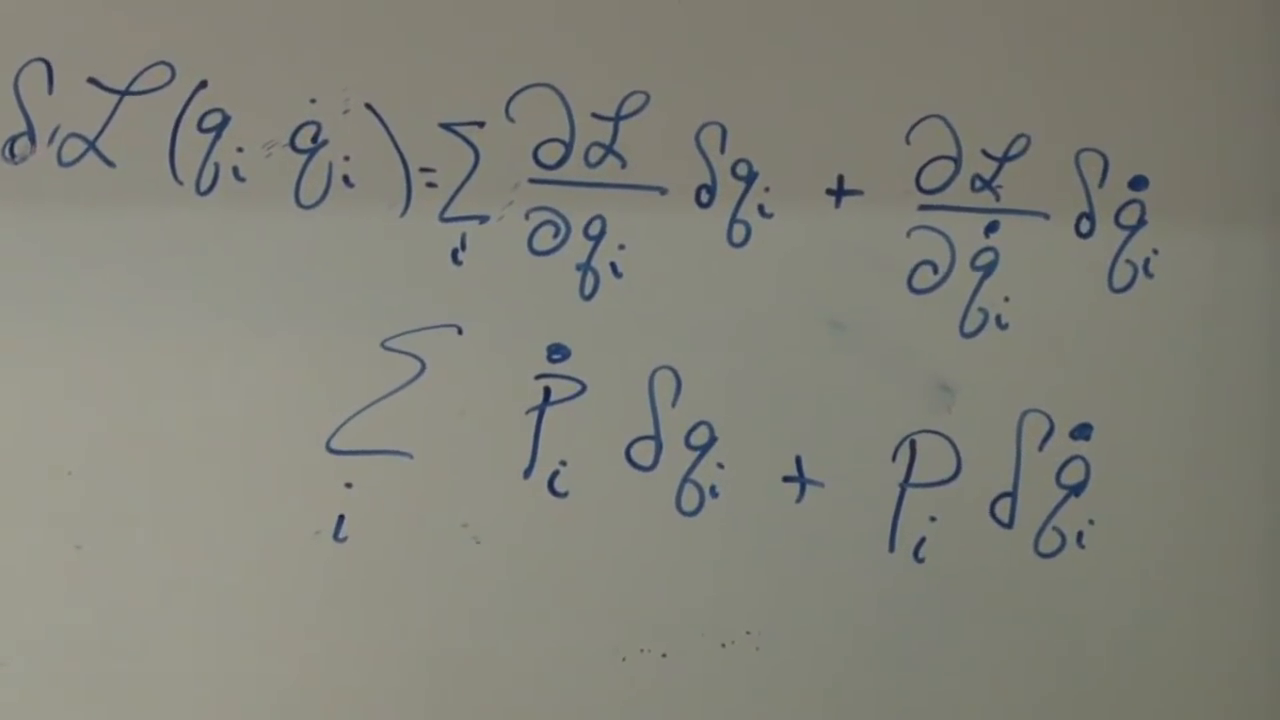
\includegraphics[width=0.84\textwidth]{lecture_04_figure_14.png}
  \caption{\(\delta L\)的两项贡献：坐标变分与
  速度变分。}
  \lectureframe{01:02:30}
\end{figure}

现在将注意力限制在物理路径上，于是欧拉--拉格朗日方程
成立。利用
\begin{equation}
  \frac{\partial L}{\partial\dot q_i}=p_i,
  \qquad
  \frac{\partial L}{\partial q_i}=\dot p_i,
  \label{eq:el-substitution-l4}
\end{equation}
我们得到
\begin{align}
  \delta L
  &=\sum_i\left(\dot p_i\,\delta q_i
                +p_i\,\delta\dot q_i\right)
  \notag\\
  &=\frac{d}{dt}\sum_i p_i\delta q_i
  =\epsilon\frac{d}{dt}\sum_i p_i f_i(q).
  \label{eq:noether-derivation-l4}
\end{align}
核心步骤只是乘积法则。

若该变换是对称变换，则\(\delta L=0\)。由于\(\epsilon\)是
任意常数因子，
\begin{equation}
  \boxed{
  \frac{d\mathcal Q}{dt}=0,
  \qquad
  \mathcal Q=\sum_i p_i f_i(q)}
  .
  \label{eq:noether-charge-l4}
\end{equation}
这就是诺特定理针对精确、
不含时的点对称性的经典力学核心。

\begin{figure}[htbp]
  \centering
  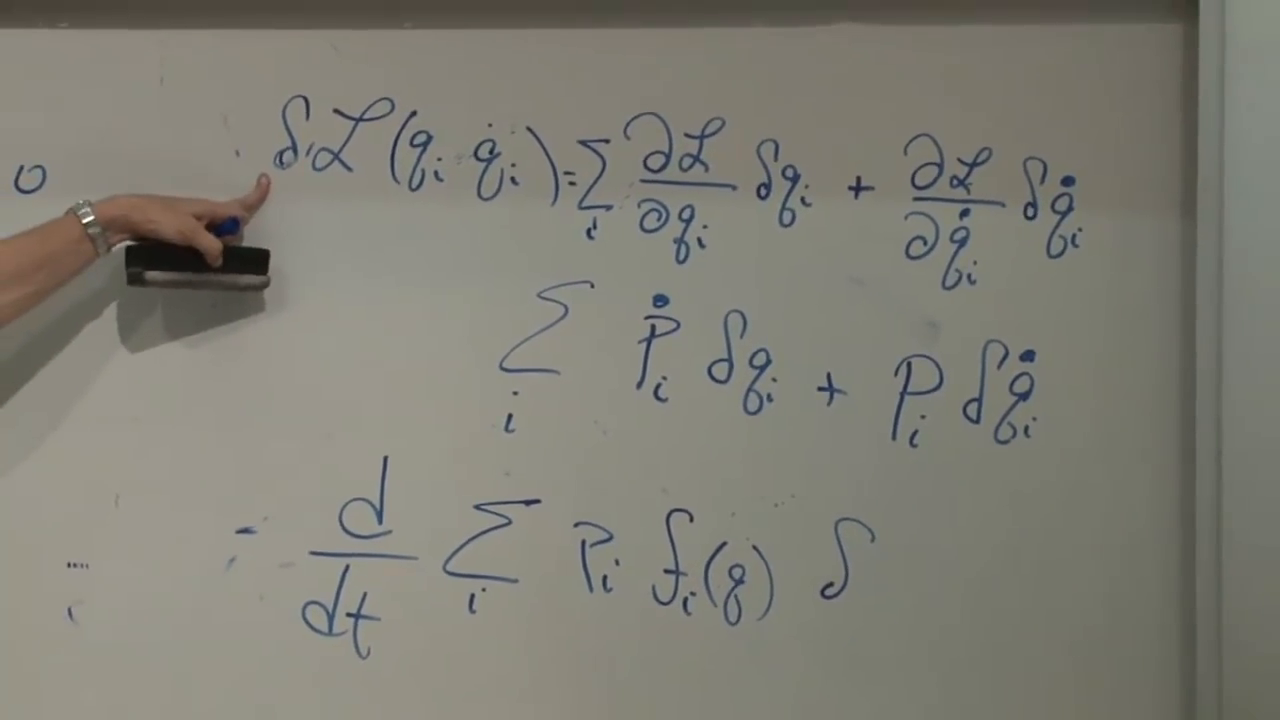
\includegraphics[width=0.84\textwidth]{lecture_04_figure_15.png}
  \caption{将\(L\)的不变性转化为
  守恒量的乘积法则步骤。}
  \lectureframe{01:05:00}
\end{figure}

\begin{classroomqa}
  \audiencequestion{在\(f_i(q)\)中，\(q\)是否还带有另一个指标？
  \lecturetimestamp{01:06:57--01:07:31}}
  \lecturerresponse{不带指标的\(q\)表示整个集合
  \((q_1,q_2,\ldots)\)。每个分量\(f_i\)可以依赖于所有这些
  坐标。例如对于旋转，\(f_x=y\)，\(f_y=-x\)。}
\end{classroomqa}

这些例子如今不再是偶然的。共同平移有
\(f_1=f_2=1\)，因此
\begin{equation}
  \mathcal Q=p_1+p_2.
  \label{eq:noether-common-p}
\end{equation}
非对称平移有\(f_1=B\)、\(f_2=-A\)，因此
\begin{equation}
  \mathcal Q=Bp_1-Ap_2.
  \label{eq:noether-ab-p}
\end{equation}
对于旋转，\(f_x=y\)且\(f_y=-x\)：
\begin{equation}
  \mathcal Q=p_xy-p_yx.
  \label{eq:rotation-charge-sign}
\end{equation}
在取向符号的意义下，这就是角动量，
\begin{equation}
  J=xp_y-yp_x.
  \label{eq:angular-momentum-l4}
\end{equation}

\begin{figure}[htbp]
  \centering
  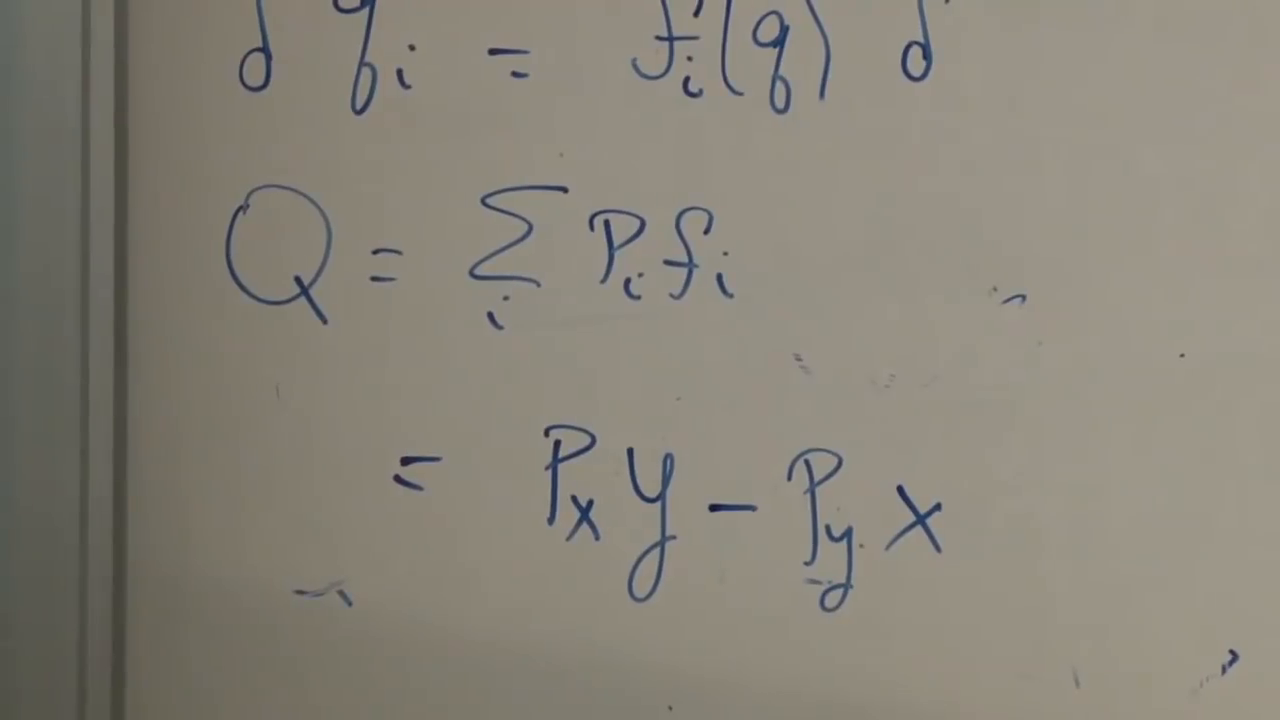
\includegraphics[width=0.82\textwidth]{lecture_04_figure_16.png}
  \caption{旋转诺特荷，在取向意义下等于平面
  角动量。}
  \lectureframe{01:11:00}
\end{figure}

对于许多相互作用粒子，将每个粒子一起旋转。此时不变性
守恒的是它们角动量之和，而不是每个粒子各自的角
动量。

\section{关于定理假设的问题}

\begin{classroomqa}
  \audiencequestion{旋转的坐标轴组是否会给\(\delta L\)引入显式的
  时间依赖？\lecturetimestamp{01:12:57--01:13:57}}
  \lecturerresponse{会。刚才给出的证明假设对称性参数
  不含时：固定的平移或固定的旋转。参数依赖于时间的
  变换会产生额外项，需要更一般的处理。}
\end{classroomqa}

\begin{classroomqa}
  \audiencequestion{板书公式中的大写\(Q\)是
  变换本身吗？\lecturetimestamp{01:14:02--01:15:58}}
  \lecturerresponse{不是。那个记号不幸地与
  坐标\(q_i\)冲突。变换是
  \(\delta q_i=\epsilon f_i(q)\)；由此得到的守恒量是
  \(\mathcal Q=\sum_i p_i f_i\)。系数\(f_i\)说明
  第\(i\)个坐标在该对称性下如何移动。}
\end{classroomqa}

能量守恒也由一种对称性生成，但是另一种对称性：
时间平移，或者说与时间零点置于何处无关。
那种情形以及哈密顿表述留待以后讨论。

\begin{classroomqa}
  \audiencequestion{实际运动能否被吸收进一个变化的
  坐标系，从而使力学变成无非是坐标
  变换？\lecturetimestamp{01:17:43--01:20:01}}
  \lecturerresponse{人们可以选择跟随某个特定
  运动的坐标，但那样变换就依赖于初始状态和
  轨迹。这里所用的对称变换是固定的，与系统
  遵循哪个解无关。运动本身更自然地在坐标与动量的
  联合空间中表示。}
\end{classroomqa}

\section{相空间中的谐振子}

取质量和弹簧常数均为1，
\begin{equation}
  L=\frac{\dot q^2}{2}-\frac{q^2}{2}.
  \label{eq:oscillator-l4}
\end{equation}
共轭动量与运动方程给出
\begin{equation}
  p=\dot q,
  \qquad
  \dot p=-q,
  \label{eq:oscillator-first-order-l4}
\end{equation}
或
\begin{equation}
  \dot q=p,
  \qquad
  \dot p=-q.
  \label{eq:oscillator-phase-flow}
\end{equation}
这些方程描述\(q\)-\(p\)平面上的匀速圆周运动。
实空间中来回振荡的振子是那个圆在
\(q\)轴上的投影：速率在\(q=0\)处最大，在转折
点处为零。

\begin{figure}[htbp]
  \centering
  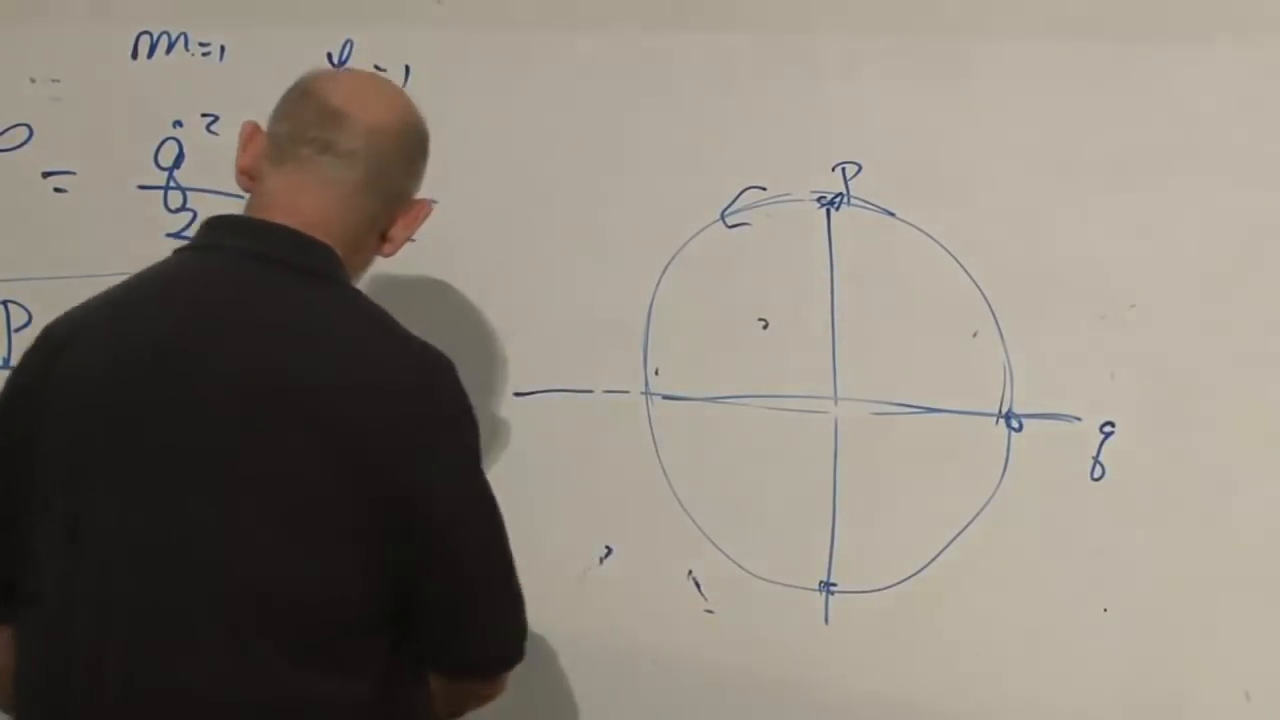
\includegraphics[width=0.82\textwidth]{lecture_04_figure_17.png}
  \caption{谐振子方程及其在
  \(q\)-\(p\)空间中的圆轨道。}
  \lectureframe{01:25:30}
\end{figure}

\begin{classroomqa}
  \audiencequestion{相空间中的圆是顺时针运行的吗？
  \lecturetimestamp{01:25:47--01:27:15}}
  \lecturerresponse{当\(p\)水平、\(q\)竖直时，是的。在
  最大的正\(q\)处，\(\dot p=-q<0\)，因此运动指向下方。
  交换两轴的位置会反转视觉上的方向，这
  解释了为什么这个约定容易被记错。}
\end{classroomqa}

式~\eqref{eq:oscillator-phase-flow}中的这一对已经类似于哈密顿
方程，但它完全是在拉格朗日力学中得到的。

\section{连续对称性与离散对称性}

\begin{classroomqa}
  \audiencequestion{对称性是否必须由无穷小笛卡尔变换来表达？\lecturetimestamp{01:27:48--01:30:31}}
  \lecturerresponse{笛卡尔坐标只是方便而已；这一证明的本质要求是连续性。有些对称性没有无穷小版本。对于偶势，反射将\(q\mapsto -q\)且\(\dot q\mapsto-\dot q\)，使\(L\)保持不变，但反射无法由任意小的反射拼装而成。因此这一经典推导不产生任何相应的守恒量。}
\end{classroomqa}

\begin{figure}[htbp]
  \centering
  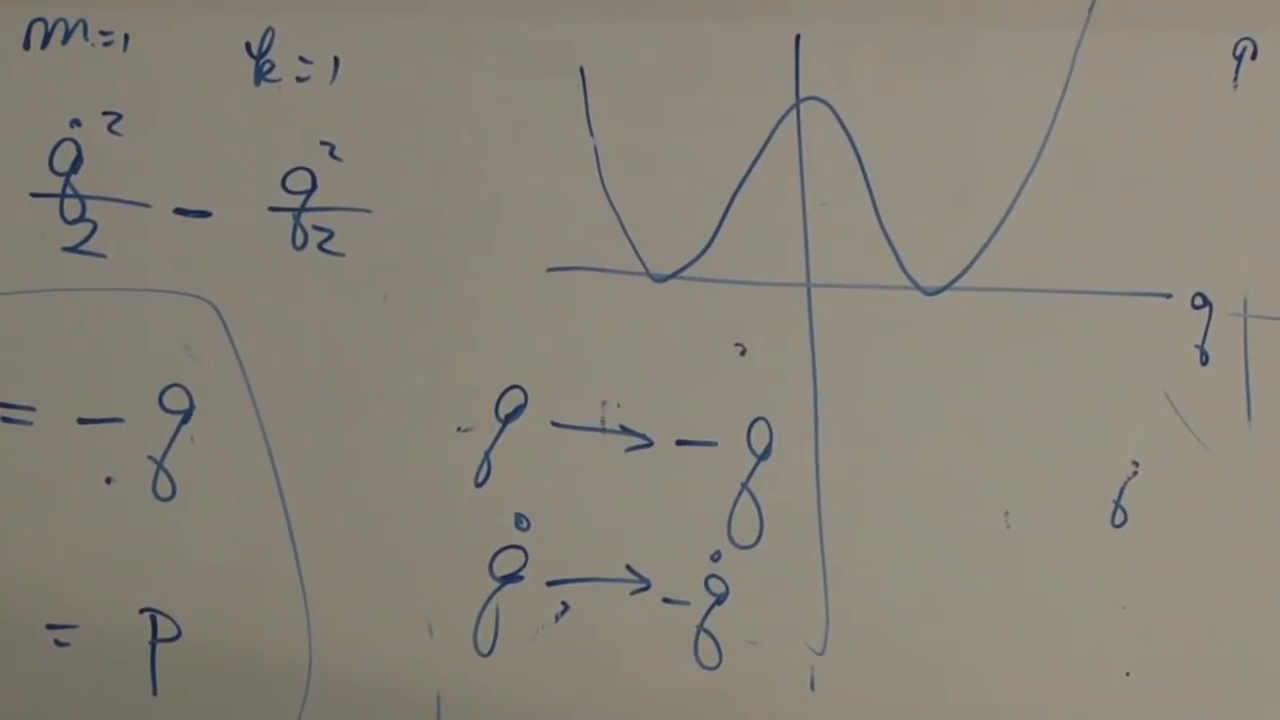
\includegraphics[width=0.82\textwidth]{lecture_04_figure_18.png}
  \caption{偶势在离散反射\(q\mapsto -q\)下不变。}
  \lectureframe{01:29:30}
\end{figure}

\begin{classroomqa}
  \audiencequestion{如果守恒量\(\mathcal Q\)非零，是否表明该变换不是一种对称性？
  \lecturetimestamp{01:30:40--01:31:30}}
  \lecturerresponse{不是。守恒量可以取任意常数值。相关的检验是\(\dot{\mathcal Q}\)。如果由某个所提出的变换导出的量不守恒，那么在该证明的假设下，那个所提出的变换就不是一种对称性。}
\end{classroomqa}

\begin{classroomqa}
  \audiencequestion{反射仍然使拉格朗日量保持不变，那么为什么它不给出守恒定律？\lecturetimestamp{01:31:34--01:32:27}}
  \lecturerresponse{仅不变性本身是可见的，但推导经过了位移的一阶项和乘积法则。反射以单个离散步骤将位形空间的一侧移到另一侧。没有无穷小生成元\(f_i\)，公式\(\mathcal Q=\sum_i p_i f_i\)便无从施展。}
\end{classroomqa}

\begin{classroomqa}
  \audiencequestion{由任意小的变换构建而成的这一性质叫什么？\lecturetimestamp{01:32:36--01:33:23}}
  \lecturerresponse{它称为\emph{连续对称性}。平移和旋转是连续的；反射是\emph{离散对称性}。}
\end{classroomqa}

\begin{classroomqa}
  \audiencequestion{如果许多无穷小步骤构成一个有限变换，被舍弃的\(O(\epsilon^2)\)误差会累积吗？
  \lecturetimestamp{01:33:23--01:36:10}}
  \lecturerresponse{无穷小不变性必须在变换所到达的每一点成立，而不仅在起点成立。将有限参数区间分成\(N\)个大小为\(\epsilon\)的步骤：累积的一阶位移为\(N\epsilon\)，而局部\(O(\epsilon^2)\)余项累积为\(N\epsilon^2=(N\epsilon)\epsilon\to0\)。这就是连续变换群所形式化的从局部到有限的结构。}
\end{classroomqa}

\begin{classroomqa}
  \audiencequestion{离散对称性在经典系统中是否物理上得以实现？\lecturetimestamp{01:36:32--01:37:25}}
  \lecturerresponse{当然。谐振子本身具有偶势\(V(q)\propto q^2\)，因此它在\(q\mapsto -q\)下不变。这样的例子很多；要点仅在于这一离散不变性不提供新的经典诺特荷。}
\end{classroomqa}

\begin{classroomqa}
  \audiencequestion{但如果连续变换和离散变换都使\(L\)保持不变，那难道不是同一个条件吗？
  \lecturetimestamp{01:37:37--01:39:18}}
  \lecturerresponse{这是同一个关于不变性的有限陈述，但不是这一证明的同一个数学输入。该证明需要一阶变分。对于反射，“一阶”没有意义，因此通向荷的方程链甚至无法启动。}
\end{classroomqa}

\begin{classroomqa}
  \audiencequestion{这在历史上与诺特定理有何关联？\lecturetimestamp{01:39:26--01:40:42}}
  \lecturerresponse{这是埃米·诺特更为普遍的定理的一个受限部分。对称性与守恒量之间的某些具体联系此前已为人所知，但诺特在二十世纪初将它们置于一个统一且极为普遍的框架之中。她的数学重要性并未得到公平的学术待遇。}
\end{classroomqa}

\begin{classroomqa}
  \audiencequestion{经典力学是否仍是一个活跃的研究课题？\lecturetimestamp{01:40:47--01:42:37}}
  \lecturerresponse{是的。这里所用的初等定理是古老的，但非线性动力学、可积系统、混沌、流体和几何力学仍是丰富的研究课题。对称性原理也远远超出经典粒子力学。}
\end{classroomqa}

\section{作用量原理为何重要}

\begin{classroomqa}
  \audiencequestion{对称性应当蕴含守恒，这有直观的理由吗？\lecturetimestamp{01:42:49--01:47:57}}
  \lecturerresponse{仅凭对称性并不能给出理由。考虑黏性阻力，
  \[
    m\ddot x=-c\dot x.
  \]
  该方程在\(x\mapsto x+\epsilon\)下不变，然而当
  \(p=m\dot x\)时，
  \[
    \dot p=-\frac{c}{m}p,
    \qquad
    p(t)=p(0)e^{-ct/m},
  \]
  因此动量衰减。这是子系统的有效方程，而不是仅对\(x\)成立的基本的稳定作用量定律。把流体分子以及闭合系统的其余部分包括进来，总动量就是守恒的。对称性与守恒是通过拉格朗日作用量原理联系在一起的，而不是仅凭一个微分方程的出现联系在一起的。}
\end{classroomqa}

\begin{figure}[htbp]
  \centering
  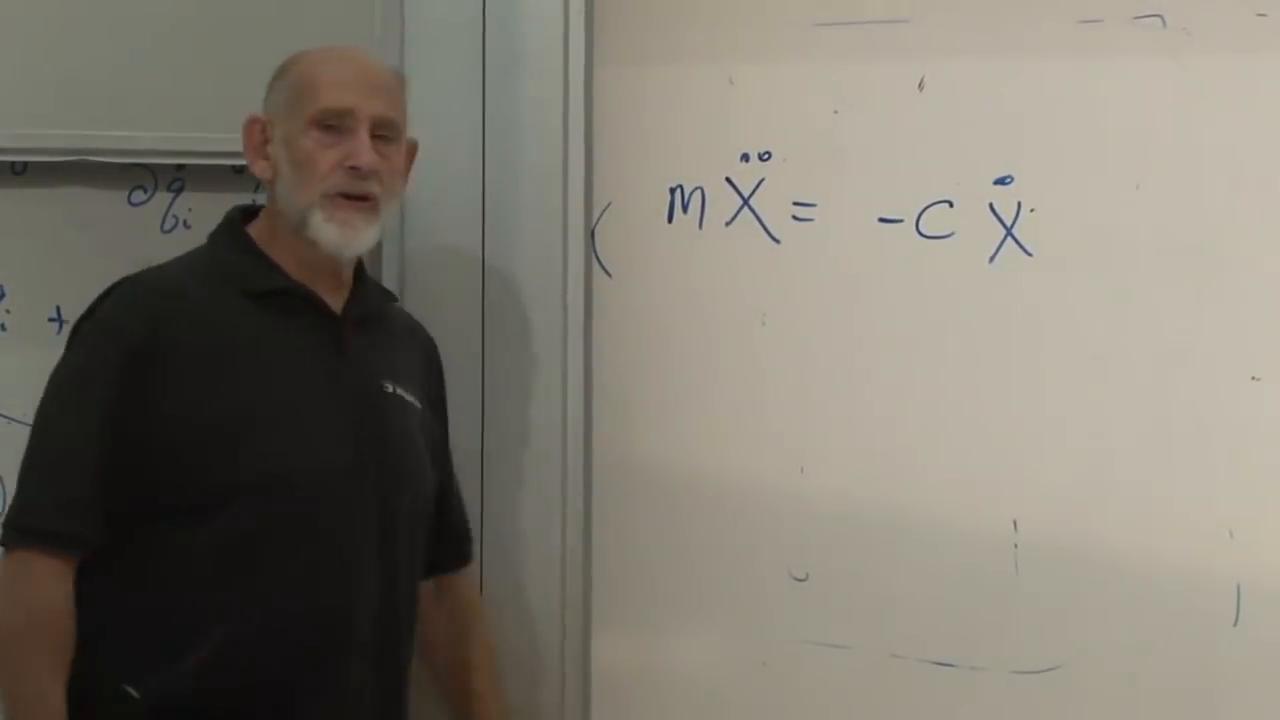
\includegraphics[width=0.65\textwidth]{lecture_04_figure_19.png}
  \caption{平移不变的黏性阻力，其约化后的粒子动量却仍然衰减。}
  \lectureframe{01:44:30}
\end{figure}

\begin{classroomqa}
  \audiencequestion{我们能否定量地说明，物理路径在什么时候不是作用量的极小值？\lecturetimestamp{01:48:08--01:51:38}}
  \lecturerresponse{真正的极小值是例外情形；作用量在路径空间中一般是鞍点。对于单位振子，
  \[
    S[q]=\frac12\int(\dot q^2-q^2)\,dt.
  \]
  狭窄而快速变化的形变会增大正的\(\dot q^2\)贡献。一个在长时间内保持略微偏离的宽形变，则可以使负的\(-q^2\)贡献占主导，从而降低作用量。因此，同一条稳定路径既有使其增大的方向，也有使其减小的方向。量子力学通过路径积分的观点给出了稳定性的更深层起源，但这一论证留待以后讨论。}
\end{classroomqa}

\begin{figure}[htbp]
  \centering
  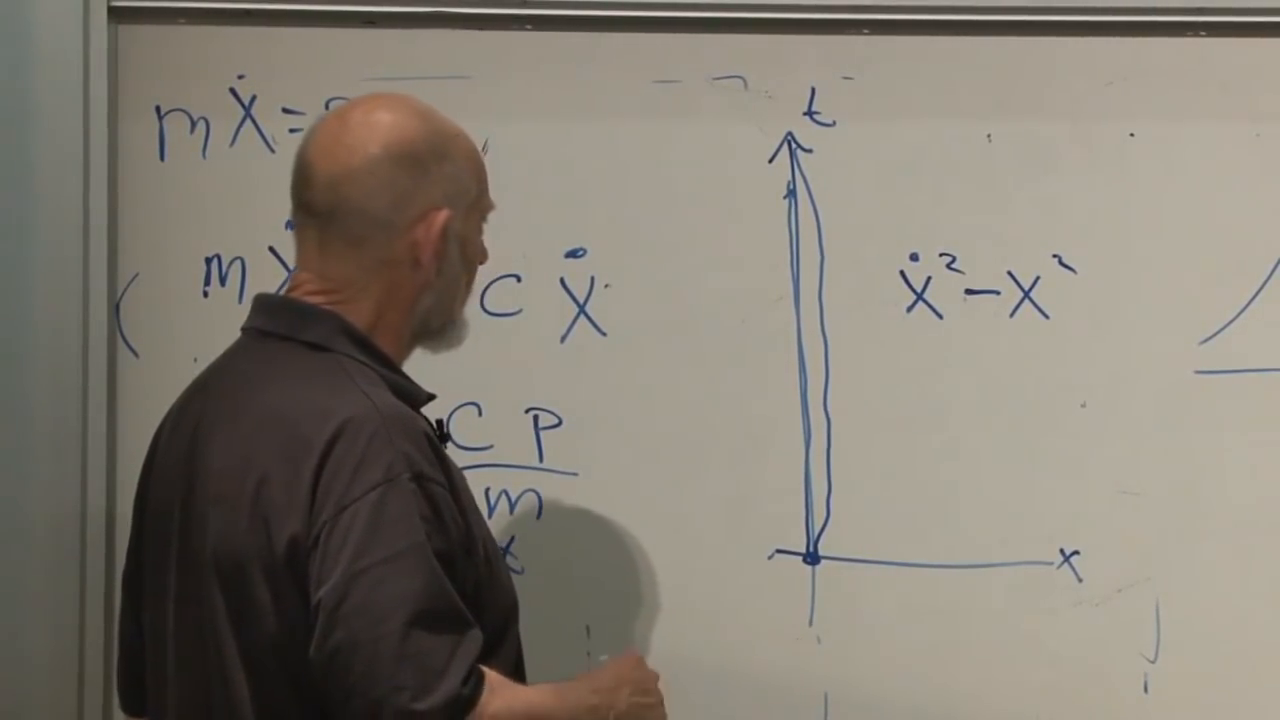
\includegraphics[width=0.80\textwidth]{lecture_04_figure_20.png}
  \caption{一条宽泛的邻近振子路径说明了，为什么稳定作用量通常是鞍点而不是极小值。}
  \lectureframe{01:50:20}
\end{figure}

\begin{classroomqa}
  \audiencequestion{连续对称性与守恒定律之间是否存在一一对应？\lecturetimestamp{01:51:44--01:52:43}}
  \lecturerresponse{在变分框架内，并在识别出等价或平凡的情形之后，这基本上就是正确的图景。每一个连续对称性都有一个荷，而守恒量一般可以追溯到对称性。精确的表述带有技术性的限定条件，因此不应轻率地使用这一宽泛的陈述。}
\end{classroomqa}

\begin{classroomqa}
  \audiencequestion{是否每一个拉格朗日量都必须具有非平凡对称性？
  \lecturetimestamp{01:52:43--01:53:23}}
  \lecturerresponse{不是。那些例子是特意选来具有对称性的。一个一般的拉格朗日量不必在任何所提出的空间变换下不变。}
\end{classroomqa}

\begin{classroomqa}
  \audiencequestion{对称性最终应当被理解为一种主动运动，还是一种被动的坐标改变？
  \lecturetimestamp{01:53:25--01:55:08}}
  \lecturerresponse{两种描述都可以做到等价，但在这里主动的描述更简洁。移动整个物理系统，并问拉格朗日量是否改变。用被动的语言，则必须说：当坐标架移动时，拉格朗日量的\emph{形式}不变。}
\end{classroomqa}

\begin{classroomqa}
  \audiencequestion{接下来是什么？\lecturetimestamp{01:55:10--01:55:35}}
  \lecturerresponse{能量守恒、它源于时间平移对称性，然后是哈密顿表述。}
\end{classroomqa}
